\chapter{定量脑电谱成分分解和特征提取的\texorpdfstring{$\xi\pi$}{ξπ}模型}
\section{研究背景}
除上一章中研究的谱常模,代表节律神经振荡的谱成分分解和参数提取对疾病诊断和神经反馈研究也十分重要,是定量脑电的关键内容。神经振荡产生电信号由神经元群的突触后电位同步放电形成电流,最后被记录为头表脑电(scalp EEG)、颅内脑电(iEEG)、皮层脑电(ECoG)和脑磁(MEG)信号\citing{buzsaki2012origin}。节律神经振荡产生的兴奋抑制形成大脑运行的传感、运动控制和认知过程。认知功能如注意、记忆、意识和脑功能失调如精神紊乱、病态心理、精神分裂,以及皮层网络的本质都可通过对神经振荡的研究进行解释\citing{buzsaki2004neuronal,uhlhaas2006neural,
uhlhaas2010abnormal,ward2003synchronous}。脑电数据的频谱曲线提供了反映大尺度神经振荡的指纹特征\citing{siegel2012spectral}。

定量脑电\citing{john1977neurometrics,da1974model,zetterberg1969estimation}在1970s被提出时分解谱成分并刻画成分特征已成为当时的热
门研究问题。L. H. Zetterberg等\citing{isaksson1981computer,wennberg1971application,zetterberg1975analogue}通过设计滤波器识别频谱中的三种成分类型并用最大似然估计法提取谱成分参数,忽略了不同谱成分在全频带上的叠加效应。随着定量脑电中计算机辅助分析诊断\citing{john1988neurometrics}出现,R. D. Pascual-marqui等\citing{pascual1988parametric}提出基于似然比检验的$\xi\alpha$模型以提取背景谱
成分$\xi$和$\alpha$节律谱成分参数,这种$\xi\alpha$模型利用Student-t型曲线\citing{walpole2011probability,fisher1925applications
,senn1994first}拟合背景非周期振荡谱成分和$\alpha$谱峰,但忽略其它频带的谱峰成分。A.K.I. Chiang等\citing{chiang2008automated}通过线性回归自动拟合$\alpha$频带上的多个子谱峰却没考虑其它频带和背景谱成分。最近,M. Haller等\citing{haller2018parameterizing}提出FOOOF模型希望拟合非周期振荡1/f过程和位于不同频带的多谱峰,但采用的最小二乘法并非基于谱估计的最优统计准则,高斯核参数估计不能鲁棒地拟合形状多变的谱成分,同时先对谱曲线作$\log_{10}$变换再分解为线性可加的谱成分意味着谱成分自然尺度上是相乘的关系,难以对结果进行解释。

我们从如下几点思考存在方法的不足:1)非周期振荡形成的背景谱成分是严格遵守1/f过程还是仅幅度单调下降\citing{abry1995wavelets}的谱曲线;2)存在的谱分解方法利用最小二乘等不具有谱估计意义的准则,采用固定参数形状的核函数如t型曲线或高斯核等参数拟合是否能鲁棒地拟合形状各异的谱成分;3)是否存在与比FOOOF中用的最小二乘更合理的准则来拟合谱成分;4)如何确定谱曲线中待拟合谱峰的个数。

为拟合形态各异的谱峰,平滑的形态回归不依赖于某种参数和形状可以更好地拟合曲线的形态\citing{eilers2005unimodal,pya2015shape}。与非
周期振荡有关的背景谱成分可能仅是单调下降的函数,各个谱峰可以看作先单调上升到谱峰再单调下降的函数。为找到谱估计的合理准则,Whittle似然利用单个频率下的傅里叶系数基于中心极限定理服从圆周复正态分布的假设,是谱估计统计学意义上的一致估计量\citing{whittle1953estimation,whittle1951hypothesis}。谱曲线拟合的关键之一是确定谱峰个数,一般可从: i)数据驱动角度,谱峰的个数就是出现在
谱曲线中的波峰的个数,被微小的波谷隔开的相近两个波峰即视为两个谱峰,这种情况下最佳的拟合通过最大似然估计获得;ii)模型驱动角度,谱峰的个数不依赖于视觉上的多少,不同频带的谱峰可能是谐波,谱峰之间可能累加或相互抵消,被稍微波谷隔开的相邻波峰可视为一个连续大谱峰,这需要从以前的神经振荡研究中获取更多的先验知识,这种情况下最小二乘法可能过拟合,这需要结合神经生理学先验知识使用组稀疏(group lasso\citing{yuan2006model})算法。本章我们发现MATLAB内置函数findpeaks能计算谱曲线中谱峰的相对重要性并能获取最小峰值高度、最小峰值宽度等参数,有助于有效识别待拟合谱成分的个数。

\begin{figure}[!h]
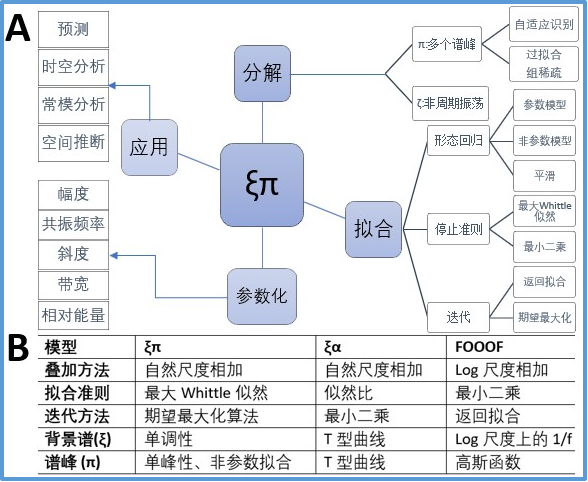
\includegraphics[width=15cm]{pic/xipi/model.png}
\caption{量化神经振荡谱曲线的$\xi\pi$模型。 A.$\xi\pi$模型综合视角,B.$\xi\pi$模型与$\xi\alpha$模型、FOOOF模型的方法比较。}
\label{7:model}
\end{figure}

量化神经振荡谱成分应该如\ref{7:model}中所示按照整体系统的观点进行。因为分解谱曲线为几个未知谱成分的累加和的过程接近于逆问题,未知谱成分是不同成分相互累加傅里叶系数的方差,利用方差成分模型和期望最大化算法\citing{Demidenko2004,mclachlan2007algorithm,zhou2019mm,
sun2016majorization}可以估计多种隐藏谱成分。谱成分中提取的如振荡幅度、共振频率、带宽和斜率等参数对某个频带下的神经振荡有解释意义。
$\xi\pi$模型具有广泛应用空间如1)用大样本正常人群数据构建头表和源空间的振荡谱特征常模;2)提取谱特征作为预测认知过程和诊断精神紊乱的生物标记物;3)用iEEG或ECoG数据基于某些有限空间采样估计全脑区的谱振荡情况\citing{owen2017towards},估计任意频率下的全脑空间谱参数
地形图。

本章我们利用Whittle似然准则和非参数拟合通过期望最大化算法来分解谱成分。我们对每个谱成分提取t型曲线有关的参数如振荡幅度、共振频率、带宽、偏斜度和斜率。这种对谱曲线的分解和提取模型称为$\xi\pi$模型,$\xi$、$\pi$分别代表非周期振荡有关的背景谱成分和周期节律振荡形成的峰峰成分
。我们发现$\xi\pi$模型的期望步骤相当于Wiener滤波器\citing{kalman1960new,Wiener1949}分离不同谱成分的频域傅里叶系数,最大化步骤中通
过最大化单调性和平滑约束的Whittle似然函数实现每个谱成分的估计。我们使用$\xi\pi$模型与FOOOF模型进行比较,利用公开的iEEG数据\citing{frauscher2018atlas},通过对谱成分参数进行高斯过程回归得到任意频率下的全脑空间谱参数成像,可能作为脑电溯源研究的谱地形图的常模参照标
准。我们在1772个电极的颅内静息态脑电数据上应用$\xi\pi$模型提取不同成分的参数,利用高斯过程回归从部分脑区的有限谱特征参数估计覆盖全脑的谱振荡得到任意频率全脑空间的谱参数地形图。与前人研究结果一致的谱参数地形图说明$\xi\pi$是一种有效的定量谱成分分解和特征提取工具。

\section{研究数据与方法}
\subsection{颅内脑电数据}
加拿大蒙特利尔神经病学研究所公开的正常静息态闭眼颅内脑电数据库\citing{frauscher2018atlas}包含加拿大和法国三家医院的106位癫痫病人
(女:54位,年龄33.1$\pm$10.8岁)接受开颅手术时被植入正常脑区的电极在非癫痫发作清醒安静闭眼状态记录的脑电数据。每个被试的电极位置不同,106位被试的电极总数达到1785。其中89位被试采用1520个立体空间穿刺电极、17位被试采用265个皮层表面条状或片状电极。左右侧大脑半球分别被覆盖1066、719个电极,大脑灰质和皮层表面的电极覆盖率分别为每立方厘米2.7和0.9个。全脑被自动划分为38个脑区,每个脑区的电极数范围为6-178个。

B. Frauscher等\citing{frauscher2018atlas}使用\href{www.bic.mni.mcgill.ca/ServicesSoftware/Services SoftwareMincToolKit}{Minctools}和IBIS架构\citing{drouin2017ibis}将颅内电极的解剖位置配准到立体空间,再将每个病人颅内手术中显示有电极位置的CT或MRI图像与病人手术前的MRI图像线性配准。手术前的MRI图像被非线性配准到ICBM152非线性对称脑模型\citing{mazziotta2001probabilistic,
fonov2011unbiased}使106病人正常脑区的电极累积为共同空间的1785个电极集。所有电极变换到共同三维空间并几乎覆盖左右半球便于对全部活动进
行组分析和可视化。如图\ref{7:ele}所示,106个被试的磁共振结构数据与电极位置被配准到共同的ICBM152\citing{mazziotta2001probabilistic,fonov2011unbiased}立体空间。
\begin{figure}[!h]
\includegraphics[width=15cm]{pic/xipi/electrodes.png}
\caption{颅内正常脑电数据集的电极分布与分区。黄色点表示电极位置。前两列从左到右从上到下分别表示左右半球的外侧和内侧视图,第三列的上下两图分别表示自头顶向下和自下向头顶的视图,最后一列表示左右半球的分区。}
\label{7:ele}
\end{figure}

我们下载到的数据集中仅有1772个电极的脑电数据。1772通道脑电数据经电生理专家视觉筛选保留至少60s无噪声的数据。颅内脑电采集使用每个电极上的局部双极参考\citing{li2018optimal},这与头表的参考问题无关。所有数据采样率均为200Hz,我们将原始数据分为2.56s的数据段,设参数时半
带宽积为3.5、最大频率为60Hz使用multitaper法\citing{thomson1982spectrum}估计功率谱。

\subsection{谱曲线分解}
我们先对脑电数据分段再对每一段作快速傅里叶变换得到傅里叶系数。如果$y_\omega$是数据段$s(s=1,...,N_s)$在频率$\omega(\omega=1,...,N_\omega)$处的傅里叶系数,$\mathbf{z}\in{\mathbb{R}^{N_k\times{1}}}$是单位向量,用以叠加$\mathbf{b}_\omega\in{\mathbb{C}^{N_k\times{1}}}$中包含的数据段s和频率$\omega$时$N_k$个成分的傅里叶系数,$\Sigma_\omega=diag(\sigma_\omega)$,$\sigma_\omega=[\sigma_\omega^1,...,\sigma_\omega^{N_k}]^T$,$\epsilon_\omega\sim{N^\mathbb{C}(0,\sigma_\epsilon)}$是所有频率上的傅
里叶系数分解残差(假设具有常数方差),那么傅里叶系数分解模型是
\begin{equation}\label{eq7.1}
y_\omega=\mathbf{z}^T\mathbf{b}_\omega+\epsilon_\omega
\end{equation}
估计的谱是所有数据段上傅里叶系数的样本方差
\begin{equation}\label{eq7.2}
s_\omega=\frac{1}{N_s}\sum_{s=1}^{N_s}y_{\omega,s}^*y_{\omega,s}
\end{equation}
指定实际计算得到的谱为$s_\omega$,理论上待拟合的谱为$\sigma_\omega$,Whittle似然\citing{pawitan1994penalized,whittle1953estimation,whittle1951hypothesis}定义为
\begin{equation}\label{eq7.3}
\ell_\omega=\sum_{\omega=1}^{N_\omega}\lbrace\log{\sigma_\omega}+\frac{s_\omega}{\sigma_\omega}\rbrace
\end{equation}

给定观测模型\eqref{eq7.1},脑电谱曲线分解转换为对傅里叶系数$\mathbf{b}_\omega$方差的估计。利用方差成分模型和期望最大化算法\citing
{mclachlan2007algorithm},未知参数的向量为$\mathbf{\theta}_\omega^{i}=(\mathbf{\sigma}_\omega^{i};\sigma_\epsilon^{i})$,则完全负$\log$似然表达式为
\begin{equation}\label{eq7.4}
\ell_c=\sum_{\omega=1}^{N_\omega}\sum_{s=1}^{N_s}\lbrace\log{\sigma}_\epsilon^{(i)}+\mathbf{\sigma}_\epsilon^{(i)-1}\mathbf{\epsilon}_\omega^{(i)*}\mathbf{\epsilon}_\omega^{(i)}+\log\lvert\Sigma_\omega^{(i)}\rvert+\mathbf{b}_{\omega,s}^{(i)*}\Sigma_\omega^{(i)-1}\mathbf{b}_{\omega,s}^{(i)}\rbrace
\end{equation}

\subsubsection{期望步骤}
\eqref{eq7.1}中$y_\omega$的方差是$c_\omega^{(i)}=\Sigma_{k=1}^{N_k}\sigma_\omega^{k(i)}+\sigma_\epsilon^{(i)}$。 根据最小模
最小二乘解和矩阵逆引理\citing{tarantola_inverse_2005},我们得到
\begin{equation}\label{eq7.5}
\mathbf{E}_{\mathbf{\theta}_\omega^{(i)}}(b_\omega^{k(i)}\mid{y}_\omega)=\sigma_\omega^{k(i)}c_\omega^{(i)-1}y_\omega
\end{equation}

显然,这里不同频谱成分频域傅里叶系数分解是一个Wiener滤波\citing{kalman1960new,Wiener1949}问题。在期望步骤,我们还可推出
\begin{equation}\label{eq7.6}
d_\omega^{k(i)}=\mathbf{E}_{\mathbf{\theta}_\omega^{(i)}}(b_\omega^{k(i)}b_\omega^{k(i)*}\mid{s}_\omega)=\sigma_\omega^{k(i)}+(s_\omega-c_\omega^{(i)})c_\omega^{(i)-2}\sigma_\omega^{k(i)2}
\end{equation}
\begin{equation}\label{eq7.7}
e_\omega^{(i)}=\mathbf{E}_{\mathbf{\theta}_\omega^{(i)}}(\epsilon_\omega^{(i)}\epsilon_\omega^{k(i)*}\mid{s}_\omega)=\sigma_\epsilon^{(i)}+(s_\omega-c_\omega^{(i)})c_\omega^{(i)-2}\sigma_\omega^{(i)2}
\end{equation}

\subsubsection{最大化步骤}
条件完全负$\log$似然函数是
\begin{equation}\label{eq7.8}
Q(\mathbf{\theta},\mathbf{\theta}^{i})=\sum_{\omega=1}^{N_\omega}\lbrace\log{\sigma_\epsilon}+\sigma_\epsilon^{-1}e_\omega^{(i)}+\sum_{k=1}^{N_k}(\log{\sigma}_\omega^k+\sigma_\omega^{k-1}d_\omega^{k(i)})\rbrace
\end{equation}
这里$\sigma_\omega^{k(i+1)}$是对$d_\omega^{k(i)}$的近似估计量,通过平滑形态约束的Whittle似然函数来拟合。

假设\eqref{eq7.1}中傅里叶系数分解残差的方差在所有频率上为常数,在最大化步骤可以计算为
\begin{equation}\label{eq7.9}
\sigma_\epsilon^{(i+1)}=\frac{1}{N_\omega}\sum_{\omega=1}^{N_\omega}e_\omega^{(i)}
\end{equation}

\subsubsection{不完全似然函数}
\begin{equation}\label{eq7.10}
\ell_{ic}=\sum_{\omega=1}^{N_\omega}\sum_{s=1}^{N_s}\lbrace\log{\sigma_\epsilon^{(i+1)}}+\frac{\epsilon_\omega^{(i)*}\epsilon_\omega^{(i)}}{\sigma_\omega^{(i+1)}}\rbrace
\end{equation}
理论上直到不完全似然函数收敛,期望最大化算法完成迭代。

\subsection{谱成分拟合}
谱成分拟合指的是谱曲线分解最大化步骤对$d_\omega^{k(i)}$的拟合。如果把所有频率对应的标量谱存为向量,我们得到$\mathbf{d}^{k(i)}=[d_1^{k(i)},...,d_\omega^{k(i)},...,d_{N_\omega}^{k(i)}]^T$和$\mathbf{\sigma}^{k(i+1)}=[\sigma_1^{k(i+1)},...,\sigma_\omega^{k(i+1)},...,\sigma_{N_\omega}^{k(i+1)}]^T$。\eqref{eq7.3}中的Whittle似然可以进一步表示为:
\begin{equation}\label{eq7.11}
\ell_\omega^{(i+1)}=\mathbf{1}^T(\log{\mathbf{\sigma}}^{k(i+1)}+\mathbf{d}^{k(i)}\bigodot{\mathbf{\sigma}^{k(i+1)-1}})
\end{equation}

使用平滑和基于单调性形态约束\citing{eilers2005unimodal,wahba1980automatic}对$\mathbf{\sigma}^k$估计的目标函数是
\begin{equation}\label{eq7.12}
\hat{\mathbf{\sigma}}^{k(i+1)}=arg\min_{\mathbf{\sigma}^{k(i+1)}}\ell_\omega^{(i+1)}+\lambda\lVert\mathbf{D}_3\mathbf{\sigma}^{k(i+1)}\rVert_2^2\quad
s.t.\;\mathbf{\sigma}^{k(i+1)}>\mathbf{0},\mathbf{D}_1\mathbf{\sigma}^{k(i+1)}<\mathbf{0}
\end{equation}

这里$\lambda$是调整平滑程度的参数,$\mathbf{D}_3$是三阶差分矩阵平滑算子,$\mathbf{D}_1$是(修正的)一阶差分矩阵梯度算子。如果$d^{k(i)}$是单调递减曲线,$\mathbf{D}_1$就是一阶差分矩阵梯度算子,对于谱峰成分$\mathbf{D}_1$在谱峰最大值左侧的元素反转正负号,即谱峰
最大值左右在梯度算子中分别具有负梯度和正梯度。在对非周期振荡谱成分$\xi$和周期节律振荡谱成分$\pi$的拟合中,调整平滑度的参数分别设为
0.1和$10^{-5}$,这些参数是经过一定范围搜索后得到,实际中是否使用精确的平滑度参数值对谱拟合的效果影响不大,主要作用在保证单调性形态约束的前提下微调平滑性。

\subsection{谱拟合误差}
对每一个电极上的谱曲线,记实际的待拟合的谱曲线为Spt、拟合的谱曲线为Fit,则拟合误差计算为
\begin{equation}\label{eq7.13}
RE = \frac{\lVert{Spt-Fit}\rVert_2}{\lVert{Spt}\rVert_2}
\end{equation}

\subsection{参数量化}
尽管在期望最大化算法的最大化步骤中我们采用非参数拟合方法拟合出单个谱成分。 为量化谱成分,我们需要逐一提取单个谱成分的参数。考虑到每一个谱成分的曲线只代表某特定频率特定电极位置的振荡事件,我们面对样本量少且群体标准偏差未知的情形近似地认为谱曲线是接近对称分布的铃形曲线,可采用Student t型的分布曲线,表示为
\begin{equation}\label{eq7.14}
f(\omega)=a/\lbrace1+[(\omega-\mu)^2/\tau]^2\rbrace^{\exp^\upsilon}
\end{equation}
这里$f$是谱成分在频率$\omega$时的功率谱值,$a$、$\mu$、$\tau$、$\upsilon$分别是该谱成分的振荡幅度、参数包括最大谱振荡幅度、共振中心
频率、幅半频带宽度和斜率。 我们采用类似与$\xi\alpha$模型\citing{pascual1988parametric}的参数提取方法。

\subsection{基于高斯过程回归绘制皮层振荡谱图}\label{ch:kriging}
从颅内某些位置的脑电谱数据中提取到的参数仅仅反映特定空间位置特定频率的振荡。为获取任意空间位置任意频率下的谱值,我们借助地学空间统计中的空间插值方法采用高斯过程回归(Kriging法)根据已知参数估计未知参数。

\subsubsection{大脑皮层空间几何学处理}
我们获取到的颅内脑电数据集仅有1772个电极的脑电数据,配准到ICBM152头模型具有238436体素点远超过电极数目1772,这样同一个电极可能位于多个相近的体素点周围。为提高从有限电极观测到全脑空间的估计准确性,我们按照MATLAB中reducepatch方法将左右脑半球的网格三角形面个数都减少到6000,空间降采样后全脑的网格顶点为$N_v=6004$个。 根据1772电极位置和全脑6004个网格顶点位置的坐标,我们找到离每个电极位置空间欧式距离最近的网格顶点。按照全脑皮层中网格顶点形成三角形面相互连接的关系首先建立权重为非0即1的对称连接矩阵6004$\times$6004,基于该连接矩阵再建立无向连接图,使用Dijkstra算法\citing{dijkstra1959note}得到全脑网格两两顶点间的最短路径长度矩阵,记为$\mathbf{G}\in{\mathbb{Z}^{N_v\times{N_v}}}$。

\subsubsection{高斯过程回归超参数选择}
记所有电极谱成分个数为$K=\sum_{e=1}^{1772}k_e$,所有谱成分所在大脑网格顶点间的最短路径长度矩阵为$\mathbf{G}_v\in{\mathbb{Z}^{K\times{K}}}$,所有谱成分共振频率间隔为$\mathbf{G}_\mu\in{\mathbb{R}^{K\times{K}}}$,所有谱成分振荡幅度为$\mathbf{a}\in{\mathbb{R}^{K\times1}}$,谱成分关于路径长度和共振频率间隔的偏差分别为$\lambda_d$、$\lambda_\mu$。谱成分分离后,我们可知每个电极的谱成分个
数k和每个谱成分的共振频率$\mu$,按照逐一电极顺序对每一个谱成分标定距离最近的大脑网格顶点$\mathbf{v}\in{\mathbb{Z}^{K\times1}}$并计算出所有谱成分共振频率间隔矩阵$\mathbf{G}_\mu$。 然后我们对所有谱成分所在网格顶点间最短路径长度矩阵和所有谱成分共振频率间隔矩阵
计算超参数,表示为
\begin{equation}\label{eq7.15}
\begin{aligned}
\mathbf{G}_v& = \mathbf{G}(v,v)^{\circ2}\\
\mathbf{W}& =\exp^{(-\frac{\mathbf{G}_v}{\lambda_d}-\frac{\mathbf{G}_\mu^{\circ2}}{\lambda_\mu})}-\mathbf{I}_K\\
\tilde{\mathbf{a}}& =\mathbf{W}\oslash{(\sum_{k=1}^K\mathbf{W}(:,k))\mathbf{1}^T}\mathbf{a}\\
(\tilde{\lambda}_d,\tilde{\lambda}_\mu)& =arg\min_{\lambda_d,\lambda_\mu}\sqrt{{\frac{\sum_{k=1}^{K}(\tilde{a}_k-a_k)}{K}}^2}
\end{aligned}
\end{equation}

\subsubsection{全脑空间谱估计与地形图绘制}
设预插值估计频率点为$\omega$,该频率点下全脑空间所有网格顶点上谱值为$\mathbf{p}_\omega$,则
\begin{equation}\label{eq7.16}
\begin{aligned}
\mathbf{G}^\prime_v& = \mathbf{G}(:,v)^{\circ2}\\
\mathbf{G}^\prime_\mu& = \mathbf{1}_{N_v}(\mathbf{\mu}^T-\omega)^{\circ2}\\
\mathbf{W}& =\exp^{(-\frac{\mathbf{G}^\prime_v}{\tilde{\lambda}_d}-\frac{\mathbf{G}^\prime_\mu}{\tilde{\lambda}_\mu})}\\
\mathbf{p_\omega}& =\mathbf{W}\oslash{(\sum_{k=1}^K\mathbf{W}(:,k))\mathbf{1}^T}\mathbf{a}
\end{aligned}
\end{equation}
利用全脑的网格顶点和三角形面信息,我们可以将任意频率下的谱值$\mathbf{p_\omega}$绘制到三维空间地形图上。
\begin{figure}[!h]
	\includegraphics[width=15cm]{pic/xipi/detect.png}
	\caption{初始化获取谱峰、谱谷的位置。Spt:从一例实际脑电数据分析得到的谱曲线,Pks:谱峰位置,Vlys:谱谷位置。}
	\label{7:detect}
\end{figure}

\section{结果与讨论}
\subsection{初始化拟合}
选择适当的初始化参数是使用期望最大化算法时减少迭代次数保证收敛到全局最优点的关键。虽然期望最大化算法是一种聚类数已知的成分混合模型,谱曲线拟合问题中每个电极的谱曲线中谱峰个数不同且共振频率位置未知,我们无法先验地确定谱成分的个数。因此进行初始化的必要任务是确定谱曲线中的待拟合成分个数。我们发现MATLAB信号处理工具箱中对测量信号进行特征提取的描述统计学函数findpeaks能较好地提取峰值。findpeaks具有最大峰值个数、最小峰值高度、最小峰值相对重要性、最小峰值高度差、最小和最大峰值宽度等参数。其中最小峰值相对重要性参数定义了谱峰下面积相对
于周围其他谱峰的重要性,本章中一般设为0.02。峰值高度和宽度可作为辅助参数,但谱曲线高度受到最大谱值的影响,我们对谱曲线按照最大谱值归一化,设最小峰值高度为0.06、最小峰值宽度为0.2。图\ref{7:detect}是用findpeaks和上述参数在一例真实脑电谱曲线中提取的谱峰和谱谷的位置。可以看出findpeaks能够较好地抓取到谱峰的位置。根据谱峰的位置、高度以及findpeaks函数返回的每一个谱峰的宽度等参数,我们可以通过t型曲线来初步拟合出每一个谱成分的曲线作为期望最大化算法中对每个谱成分的初始拟合。

\subsection{\texorpdfstring{$\xi\pi$}{ξπ}与FOOOF模型效果比较}
谱曲线拟合和成分特征提取的方法中,Zetterberg等的方法\citing{isaksson1981computer,wennberg1971application,
zetterberg1975analogue}是基于滤波器设计,Pascual的方法\citing{pascual1988parametric}只能拟合$\alpha$谱峰和背景非谱峰成分,
Chiang的方法\citing{chiang2008automated}只对$\alpha$频带的多个子谱峰进行拟合,只有Haller等的方法FOOOF\citing{haller2018parameterizing}可拟合多种谱峰和背景非谱峰成分。因此,我们比较$\xi\pi$与FOOOF模型的拟合效果。
\begin{figure}[!h]
	\includegraphics[width=15cm]{pic/xipi/comp.png}
	\caption{$\xi\pi$模型与FOOOF模型的拟和效果比较。 Spt: 原始谱曲线,$\xi\pi$:本文提出的模型,FOF:FOOOF模型\citing{haller2018parameterizing}。A.模型总体拟合效果比较,B.背景振荡拟合效果比较,C.谱峰拟合效果比较,D.使用FOF Python工具包拟合结
	果原图,纵坐标的Power实际上是对原始谱曲线求$log_{10}$后的值。}
	\label{7:comp}
\end{figure}

FOOOF模型先对实际谱数据作$log_{10}$变换再对背景振荡和谱节律成分按叠加模型分别拟合。与之不同,$\xi\pi$模型直接在原始自然尺度的谱曲
线上进行分解和拟合。为与FOOOF工具包的原始结果形成对比,我们将$\xi\pi$自然尺度上的拟合结果画到$\log_{10}$尺度。
图\ref{7:comp}D是使用FOOOF模型\href{https://github.com/fooof-tools/fooof/tree/master/fooof}{基于Python语言的工具包}对一例实际
脑电谱数据拟合输出的原图。$\xi\pi$模型与FOOOF模型的效果比较分别表示在图\ref{7:comp}ABC中,依次是全模型对谱曲线的整体拟合效果、对背景
非周期振荡曲线的拟合效果和对节律周期振荡谱峰成分的拟合效果。图\ref{7:comp}A表明$\xi\pi$模型比FOOOF模型拟合效果更好,拟合出的谱曲线基
本和实际相重合,相比,FOOOF模型拟合出的曲线严重偏离实际谱曲线。图\ref{7:comp}B中$\xi\pi$模型拟合出的非周期背景振荡谱曲线较好地吻合实际谱曲线的背景振荡非谱峰位置,然而FOOOF模型甚至在低频处拟合出比实际高很多、在高频处比实际低很多的曲线。$\xi\pi$模型与FOOOF对周期节律
振荡谱成分的效果对比说明$\xi\pi$模型在全频带上都有信号,特别是谱峰幅度小于1时也随频率变化,谱峰的位置较好地出现在如图\ref{7:detect}中自然尺度谱峰的下方位置,然而FOOOF模型先对谱曲线做$log_{10}$变换再进行拟合,在$log_{10}$尺度拟合出的谱峰成分在谱峰周围都为0。总体
上$\xi\pi$拟合出的谱曲线较好地保持实际谱曲线的细节变化,非周期的背景振荡谱成分是单调下降的曲线,对于谱峰成分拟合,在全频带上都拟合出随频率变化体现几个共振频率谱峰的叠加趋势,这是$\xi\pi$模型使用非参数拟合和单调性约束的结果;然而FOOOF模型拟合曲线表现出较强的平滑性,无论背景振荡还是节律谱成分振荡曲线拟合都明显表现出某种形状,这种形状由高斯核确定。显然对本例非对称形状且左右瓣凹凸性不一致的谱峰,FOOOF对每个谱峰拟合出的左右瓣都严格对称且向外凸,$\xi\pi$模型的非参数拟合得到比FOOOF模型更符合实际的效果。

\subsection{\texorpdfstring{$\xi\pi$}{ξπ}模型的拟合过程与分解效果}
\begin{figure}[!h]
	\includegraphics[width=15cm]{pic/xipi/allinone.png}
	\caption{$\xi\pi$模型的迭代和总体分离效果。A.迭代拟合,Init:根据findpeaks进行初始化的结果,i=1、5、10表示第1、5、10次迭代。 
	B.负log似然函数随迭代次数的变化。C.最终总体拟合与分离效果,$\alpha_1$、$\alpha_2$、$\beta_1$、$\beta_2$表示$\alpha$、$\beta$频带上的第1、2个谱峰成分。}
	\label{7:allinone}
\end{figure}

为进一步了解$\xi\pi$模型的拟合过程和成分分解效果,图\ref{7:allinone}AB表示对与上节相同实际脑电谱数据的迭代拟合结果和负似然函数变化
。 从B中可知负似然函数随迭代次数增多下降,表明模型使用期望最大化算法进行迭代拟合和分解的有效性。实际模型计算中我们发现负似然函数有时难以收敛但10次左右迭代后拟合出谱曲线已与实际谱曲线较好地吻合。负似然函数还未收敛的原因是模型还在试图拟合某些未完全吻合的细节,但这些未拟合好的细节正是模型中的单调性形态约束造成的,过度追求目标函数收敛已经无太大意义。拟合效果随迭代变化趋势如图\ref{7:allinone}A中所示
,易看出根据findpeaks进行初始化的结果已接近实际谱曲线,$\xi\pi$模型期望最大化算法的作用是对初始化结果进行迭代调整。根据经验,如果负似然函数迭代超过50次还不收敛,我们会终止迭代取所有迭代中拟合出的谱曲线与实际谱曲线相对误差(RE)最小值的拟合。图\ref{7:allinone}B表示对该实际脑电谱曲线的总体拟合和分解效果,蓝色原始谱曲线几乎被深蓝色拟合出的谱曲线完全覆盖,深蓝色拟合出的谱曲线是表示非周期背景振荡的$\xi$与表示周期节律振荡的$\pi$($\theta$、$\alpha_1$、$\alpha_2$、$\beta_1$、$\beta_2$)成分线性叠加的结果。$\xi\pi$模型的主要目标
之一是将实际谱曲线分离为非周期振荡和若干代表节律振荡的谱峰成分。


\subsection{颅内脑电谱参数提取}
我们对1772个电极的脑电信号进行谱分析,根据student t型曲线提取出谱成分振荡最大幅度$a$、谱成分共振中心频率$\mu$、谱成分幅半频带宽度$
\tau$和斜率$\upsilon$。虽然电极谱曲线中成分个数不同,但根据\cite{frauscher2018atlas}文中报道的结果我们先验地设置谱曲线中的最大成分
数不超过15。图\ref{7:para}A中左右两图分别表示$\xi\pi$模型对1772个电极谱曲线拟合相对误差随谱曲线成分个数的变化和1772个电极谱曲线拟合
误差关于电极数的归一化后直方图分布。从图\ref{7:para}A左图中可看出极少比例电极上谱曲线仅具有非周期振荡不具有节律振荡,大部分电极上具有
2-6个谱成分,还有一部分具有7个及以上谱成分。图\ref{7:para}A右边直方图表明所有电极上拟合误差在0.1(10\%)左右,对应左图中较亮颜色(红黄
白色)处的RE,说明总体上$\xi\pi$模型拟合效果较好。

图\ref{7:para}中BC两行自左向右分别表示节律周期振荡谱峰成分$\pi$和非周期振荡背景谱成分$\xi$中最大振荡幅度$a$随共振频率$\mu$的直方图、
最大振荡幅度$a$随振荡频率幅半带宽$\tau$的直方图、斜率$\upsilon$随振荡频率幅半带宽$\tau$的直方图。从BC两行的第一列上下两图可看出节律振荡在8、12、22Hz左右形成较强谱峰,非周期背景振荡在最小频率分辨率点0.39Hz处具有最大振荡幅值,这与文献\cite{frauscher2018atlas}报道的谱峰频率位置相吻合,以及与非周期背景振荡在最低频率点具有最大振荡幅度的认识相一致;从BC两行的第二列的上下两图中观察发现非周期背景谱成分和节律谱峰成分的最大振荡幅值都随带宽增加而下降,这与物理学中的振荡谱能量呈现1/f类型\citing{abry1995wavelets}的幂律分布相吻合
;BC两行的第三列两图表示斜率都随振荡带宽增加而上升但节律周期振荡斜率在大多数情况下大于非周期背景振荡的斜率,这一点与\cite{pascual1988parametric,amador1989structure,amador1990spatiotemporal}等论文的结果类似;这也和周期节律振荡与系统中不稳定的随机突发性振荡事件有关、背景非周期振荡与系统中稳定的可能是噪声活动有关,不稳定的随机突发振荡事件的谱曲线类似于窄带脉冲具有远大于稳定非周期噪声的宽带振荡的斜率。
\begin{figure}[!h]
\includegraphics[width=15cm]{pic/xipi/para.png}
\caption{1772个电极谱拟合与参数提取。A行:左图表示拟合误差随拟合出的谱成分个数变化的直方图,右图表示1772个电极上谱成分的拟合误差直方图;B行表示谱峰$\pi$成分拟合情况,左图是$a$随$\mu$的直方图分布,中图是$\mu$随$\tau$的直方图分布,右图是$\upsilon$随$\tau$的直
方图分布;C行表示背景振荡$\xi$的拟合情况。 所有直方图的颜色尺度相同。}
\label{7:para}
\end{figure}

\subsection{全脑空间谱地形图}
对1772个电极上谱曲线拟合并提取成分参数,我们采用描述在\ref{ch:kriging}一节中基于高斯过程回归的方法估计任意频率全脑空间任意网格顶
点位置上的振荡谱值。我们分别估计传统频带$\delta$(1-3Hz)、$\theta$(4-7Hz)、$\alpha$(8-12Hz)、$\beta$(16-30Hz)的最大振荡谱值分布,
并根据全脑空间的网格顶点和三角形面信息将分布结果以2、5、10、26Hz为例画在图\ref{7:map}中的大脑皮层上。图\ref{7:map}的每一列对应一个频带,自上向下分别是顶测、左侧、右侧视图。不同频带的空间地形图的颜色尺度不同,从低频到高频颜色尺度的最大最小值范围逐渐减小。我们发现$\delta$节律振荡主要分布在前额叶、左侧枕叶和双侧颞叶,$\theta$节律振荡主要分布在右侧上额回、右侧辅助运动区、右侧前后中央回、左侧枕叶和左侧前额
叶,$\alpha$节律振荡主要分布在左右双侧颞叶、左右双侧枕叶和左侧顶叶,$\beta$节律振荡主要分布在左右双侧上额回、左右双侧前后中央回和左
侧辅助运动区,集中在前额叶和顶叶,呈现双侧对称分布。 总体上,$\delta$、$\theta$、$\beta$节律的分布更为分散,$\alpha$节律的分布主要
集中在后中央回以下的顶枕叶,但全部枕叶并非只有$\alpha$节律,部分枕叶区域可能出现$\delta$和$\theta$节律。这些结果与报道在\cite{gastaut1949enregistrement,jasper1949electrocorticograms,sem1953depth,chatrian1960depth,sem1956electroencephalographic,perez1962electrographic,graf1984electrocorticography,frauscher2018atlas}等论文中的结果相吻合。基于$\xi\pi$模型和高斯过程回归的方法,我们对颅内部分位置有限空间采样的脑电信号谱曲线分解提取出各个谱成分的参数进行频率和空间位置上的插值,得到与文献\citing{frauscher2018atlas}等相一致的结果,这种频率和大脑空间位置两个维度的高分辨率神经振荡节律谱地形图可作为正常脑电的源空间谱常模,可能为源空间的定量脑电分析提供一种基准。
\begin{figure}[!h]
	\includegraphics[width=15cm]{pic/xipi/map.png}
	\caption{全脑空间谱地形图。从左到右分别是$\delta$(2Hz)、$\theta$(5Hz)、$\alpha$(10Hz)、$\beta$(26Hz)处的谱地形图,前三行自上
	向下分别是顶、左、右侧视图,各个频带具有不同颜色尺度。}
	\label{7:map}
\end{figure}

% \section{讨论}
% There are a few problems remained to solve: (1) Add the constraint σ > 0 when using Whittle likelihood at
% ordinary scale. (2) To tune the smoothing parameter, how to calculate the degree of freedom of a
% nonparametric fitting? divergence of MLE (Monto Carlo)? (3) Can Whittle likelihood be transformed into a least
% square, via series expansion or by log transformation (check the expansional family)? (4) Organize the Bayesian
% and spectrum papers in Mendeley. (5) Review Bayesian analysis, projection estimator, Wahba smoothing and
% Whittle likelihood.
% The developer version of the Xi rhythms toolbox is at https://github.com/ShiangHu/SCMOPT.git.
% author/funder. 

\section{本章小结}
本章我们提出$\xi\pi$模型,它基于最大Whittle似然估计和单调性形态约束的非参数拟合,能有效分解谱曲线中多个谱峰与非周期振荡谱并提取谱成
分特征。该模型与前人方法的主要不同在于使用基于Whittle似然这种更具有谱估计统计学意义的准则,利用不完全数据的方差成分模型和期望最大化算法对每一个成分的拟合首次采用单调性约束的非参数拟合。我们应用$\xi\pi$模型取得了比基于高斯核的FOOOF模型更好的估计,证明FOOOF模型在$\log_{10}$尺度进行参数拟合的缺点。我们应用$\xi\pi$模型到1772正常颅内脑电数据集上得到一种高频率空间分辨率的全脑空间节律振荡谱地形图
,可能作为源空间定量脑电谱分析的参照基准。